% DO NOT COMPILE THIS FILE DIRECTLY!
% This is included by the other .tex files.
\section*{Primeira parte}
\begin{frame}[t,plain]
\titlepage
\end{frame}
%%%%%%%%%%%%%%%%%%%%%%%%%%%%%%%%%%%
%%%%%%%%%%%%%%%%%%%%%%%%%%%%%%%%%%%
\begin{frame}{Bem-vindas (os)!}
Este é um curso de 60 (sessenta) horas sobre Inferência Estatística.

\textbf{Princípios:}
\begin{itemize}
  \item[$\triangle$] Em uma palavra:~\underline{Liberdade};
  \item[$\triangle$] Construção conjunta do conhecimento;
  \item[$\triangle$] Pontualidade na entrega das tarefas;
  \item[$\triangle$] Participação em aula;
\end{itemize}

\textbf{Burocracia:}
\begin{itemize}
 \item[$\square$] Horário de atendimento: Segundas e quartas de 14:30h a 15:30h.
 \begin{itemize}
  \item  Por favor, mandar e-mail com antecedência de 24h para marcar;
  \end{itemize} 
 \item[$\square$] Podem escrever por e-mail (ou carta) quando quiserem;
 \item[$\square$] Teremos duas avaliações (A1 e A2) e 4 (quatro) trabalhos ($T_i$, $i = 1,2,3,4$).
 Trabalhos valerão 20\% do grau final.
 \item[$\square$] Nota final será $\text{NF} := \frac{3A_1 + 7A_2}{10} + \sum_{i=1}T_i$.
\end{itemize}
\end{frame}
%%%%%%%%%%%%%%%%%%%%%%%%%%%%%%%%%%%
%%%%%%%%%%%%%%%%%%%%%%%%%%%%%%%%%%%
\begin{frame}{Revisão de Teoria da Probabilidade}
\begin{itemize}
 \item Desigualdade de Markov;
 \item Desigualdade de Chebychev;
  \item Convergência;
 \item Lei(s) dos grandes números;
 \item Teorema(s) Central(is) do Limite;
\end{itemize}
\end{frame}
%%%%%%%%%%%%%%%%%%%%%%%%%%%%%%%%%%%
%%%%%%%%%%%%%%%%%%%%%%%%%%%%%%%%%%%
\begin{frame}{Desigualdade de Markov\footnote{Em homenagem a Andrey Andreyevich Markov (1856–1922).}}
Seja $X$ uma variável aleatória não-negativa e $t > 0$.
Então
\begin{equation}
 \label{eq:Markov_ineq}
 \pr(X \geq t) \leq \frac{E[X^n]}{t^n}.
\end{equation}
\textbf{Prova:} Assumindo que $X$ é absolutamente contínua, escrever $E[X]$ explicitamente e usar linearidade e monotonicidade da integral.
Para $n = 1$ e $X$ discreta, ver De Groot, página 349, Teorema 6.2.1 $\qed$
\end{frame}
%%%%%%%%%%%%%%%%%%%%%%%%%%%%%%%%%%%
\begin{frame}{Desigualdade de Chebychev\footnote{Em homenagem a Pafnuty Lvovich Chebyshev (1821--1894).}}
Seja $Y$ uma variável aleatória com média $E[Y] =: \mu$ e variância $\vr(Y) =: \sigma^2$, ambas finitas.
Mais uma vez, $t>0$.
Então
\begin{equation}
 \label{eq:Chebychev_ineq}
 \pr(|Y-\mu| \geq t) \leq \frac{\vr(Y)}{t^2}.
\end{equation}
\textbf{Prova:} Notar que $E[(Y-\mu)^2] = \sigma^2$ e aplicar Markov.
Ver De Groot, página 349, Teorema 6.2.2 $\qed$
\end{frame}
%%%%%%%%%%%%%%%%%%%%%%%%%%%%%%%%%%%

%%%%%%%%%%%%%%%%%%%%%%%%%%%%%%%%%%%
\begin{frame}{A média amostral}
Considere uma~\textbf{amostra aleatória} $X_1, X_2, \ldots, X_n$, $n \in \mathbb{N}$ de variáveis aleatórias de uma mesma distribuição com média $E[X_i] = \mu$ e variância $\vr(X_i) = \sigma^2$.
\begin{defn}
 \textbf{Média amostral}. A média amostral de $X_1, X_2, \ldots, X_n$ é
 \begin{equation}
  \label{eq:sample_mean}
  \bar{X}_n := \frac{1}{n} \sum_{i = 1}^n X_i.
 \end{equation}
\end{defn}

\begin{theo}
\label{thm:iid_properties}
Sejam  $X_1, X_2, \ldots, X_n$ variáveis aleatórias independentes e identicamente distribuídas, com média $\mu$ e variância $\sigma^2$.
Temos que (i) $E[\bar{X}_n] = \mu$ e (ii) $\vr(\bar{X}_n) = \frac{\sigma^2}{n}$.
\end{theo}
\textbf{Prova:} Para (i), usar a linearidade da esperança e o fato de as variáveis serem identicamente distribuídas -- note a falta de menção à independência.
Para (ii), usar a soma das variâncias de variáveis idependentes, além do fato de serem identicamente distribuídas.
Ver De Groot, página 350, Teorema 6.2.3.
\end{frame}
%%%%%%%%%%%%%%%%%%%%%%%%%%%%%%%%%%%
\begin{frame}[allowframebreaks,fragile]{Exemplo: determinando o tamanho de amostra}
Vamos estudar o exemplo 6.2.3 de De Groot.
Suponha  que uma moeda justa é lançada $n$ vezes.
Seja $X_i$ a variável aleatória que é $1$ se o $i$-ésimo lançamento dá cara e $0$ caso contrário.
Considere $\bar{X}_n = \frac{1}{n} \sum_{i=1}^n X_i$.
\begin{pergunta}
Quantos lançamentos devemos fazer para que 
$$ \pr(0.4 \leq \bar{X}_n \leq 0.5) \geq 0.7\: ?$$
\end{pergunta}
\textbf{Resolução:} Primeiro, faça $S_n = \sum_{i=1}^n X_i$ e deduza que $E[S_n] = np = n/2$ e $\vr(S_n) = n p(1-p) = n/4$.
Agora:
$$ \pr(0.4 \leq \bar{X}_n \leq 0.5) = \pr\left(\frac{4n}{10} \leq S_n  \leq \frac{6n}{10} \right).$$
Subtraia $E[S_n]$ dos dois lados da desigualdade para obter
$$ \pr\left(\frac{4n}{10} \leq S_n  \leq \frac{6n}{10} \right) = \pr \left(\left|S_n - \frac{n}{2} \right|\leq \frac{n}{10} \right) .$$
Note que, usando a desigualdade de Chebychev, temos uma cota superior para 
$$\pr \left(\left|S_n - \frac{n}{2} \right|\geq \frac{n}{10} \right) = 1 - \pr \left(\left|S_n - \frac{n}{2} \right|\leq \frac{n}{10} \right).$$
Portanto
$$\pr \left(\left|S_n - \frac{n}{2} \right|\geq \frac{n}{10} \right) \leq \frac{100}{4n}$$ 
e então
$$ \pr(0.4 \leq \bar{X}_n \leq 0.5) = \pr \left(\left|S_n - \frac{n}{2} \right|\leq \frac{n}{10} \right) \geq 1 - \frac{25}{n}.$$
Resolvendo $ 1 - 25/n = 0.7$ obtemos $n \geq 84$.

\framebreak
Agora, vamos usar o que sabemos~\textbf{especificamente} sobre este problema.
Usando uma tabela de probabilidades binomiais ou rodando um programa como:
\begin{minted}{R}
calcula_p <- function(n){
  prob <- pbinom(q = round(0.6*n), size = n, p = .5) 
  - pbinom(q = round(0.4*n)-1, size = n, p = .5)
  return(prob)
}
n <- 10
p <- calcula_p(n)
alvo <- 0.7
erro <- (p-alvo)^2
while(erro > .001){
  n <- n + 1
  p <- calcula_p(n)
  erro <- (p-alvo)^2
  if(n > 10000) break
}
\end{minted}
obtemos \verb|n = 15| e \verb|p = 0.6982422|.

\textbf{Conclusão}: a desigualdade de Chebychev é~\underline{frouxa}, isto é, ela dá uma cota superior para a probabilidade de interesse, mas essa cota pode ser muito maior do que o valor exato.
Por outro lado, a desigualdade é válida para~\underline{qualquer} variável aleatória cuja variância exista e seja finita.

\begin{ideia}
\label{idea:no_free_lunch}
 \textbf{Sem almoço grátis}.
 Se uma técnica ou resultado é muito geral, isto é, se aplica a muitas situações, há grandes chances de não fornecer uma resposta muito precisa.
 O contrário também é verdadeiro: se desenvolvemos uma técnica elaborada para uma classe restrita de problemas, geralmente vamos obter respostas precisas, mas nossa técnica não será aplicável a muitos tipos de problemas.
 Em Estatística não existe almoço grátis.
\end{ideia}

\end{frame}
%%%%%%%%%%%%%%%%%%%%%%%%%%%%%%%%%%%
\begin{frame}{Convergência}
\begin{defn}
\label{defn:weak_convergence}
\textbf{Convergência em probabilidade}.
Dizemos que uma sequência de variáveis aleatórias~\textit{converge em probabilidade} para $b$ se, para todo $\epsilon > 0$, temos
\begin{equation}
 \nonumber
 \lim_{n\to\infty} \pr\left(|Z_n-b| < \epsilon \right) = 1.
\end{equation}
Neste caso, escrevemos $Z_n \xrightarrow{\text{p}} b$.
\end{defn}
Em algumas situações, chamamos a convergência em probabilidade de convergência fraca.
\end{frame}
%%%%%%%%%%%%%%%%%%%%%%%%%%%%%%%%%%%
\begin{frame}{Lei(s) dos Grandes Números (LGN)}

A lei fraca dos grandes números é um resultado fundamental da Teoria de Probabilidade, extremamente útil em Estatística.
\begin{theo}
\label{thm:WLLN}
\textbf{Lei Fraca dos Grandes Números}.
Sejam  $X_1, X_2, \ldots, X_n$ variáveis aleatórias independentes e identicamente distribuídas, com média $\mu$ e variância $\sigma^2$.
 Então
 $$ X_n \xrightarrow{\text{p}} \mu.$$
\end{theo}
\textbf{Prova:}
Usando o teorema~\ref{thm:iid_properties} e a desigualdade de Chebychev, temos
$$ \pr\left( |\bar{X}_n - \mu| < \epsilon\right) \geq  1 - \frac{\sigma^2}{n\epsilon^2},$$
e, portanto,
$$ \lim_{n\to\infty} \pr\left( |\bar{X}_n - \mu| < \epsilon\right) = 1. \: \qed$$
\end{frame}
%%%%%%%%%%%%%%%%%%%%%%%%%%%%%%%%%%%
\begin{frame}{LGN: exemplo}
$X_1, \ldots, X_n \sim \operatorname{Beta}(3, 2)$.
$E[X] = \alpha / (\alpha + \beta) = 3/5$.
\begin{figure}[!ht]
\begin{center}
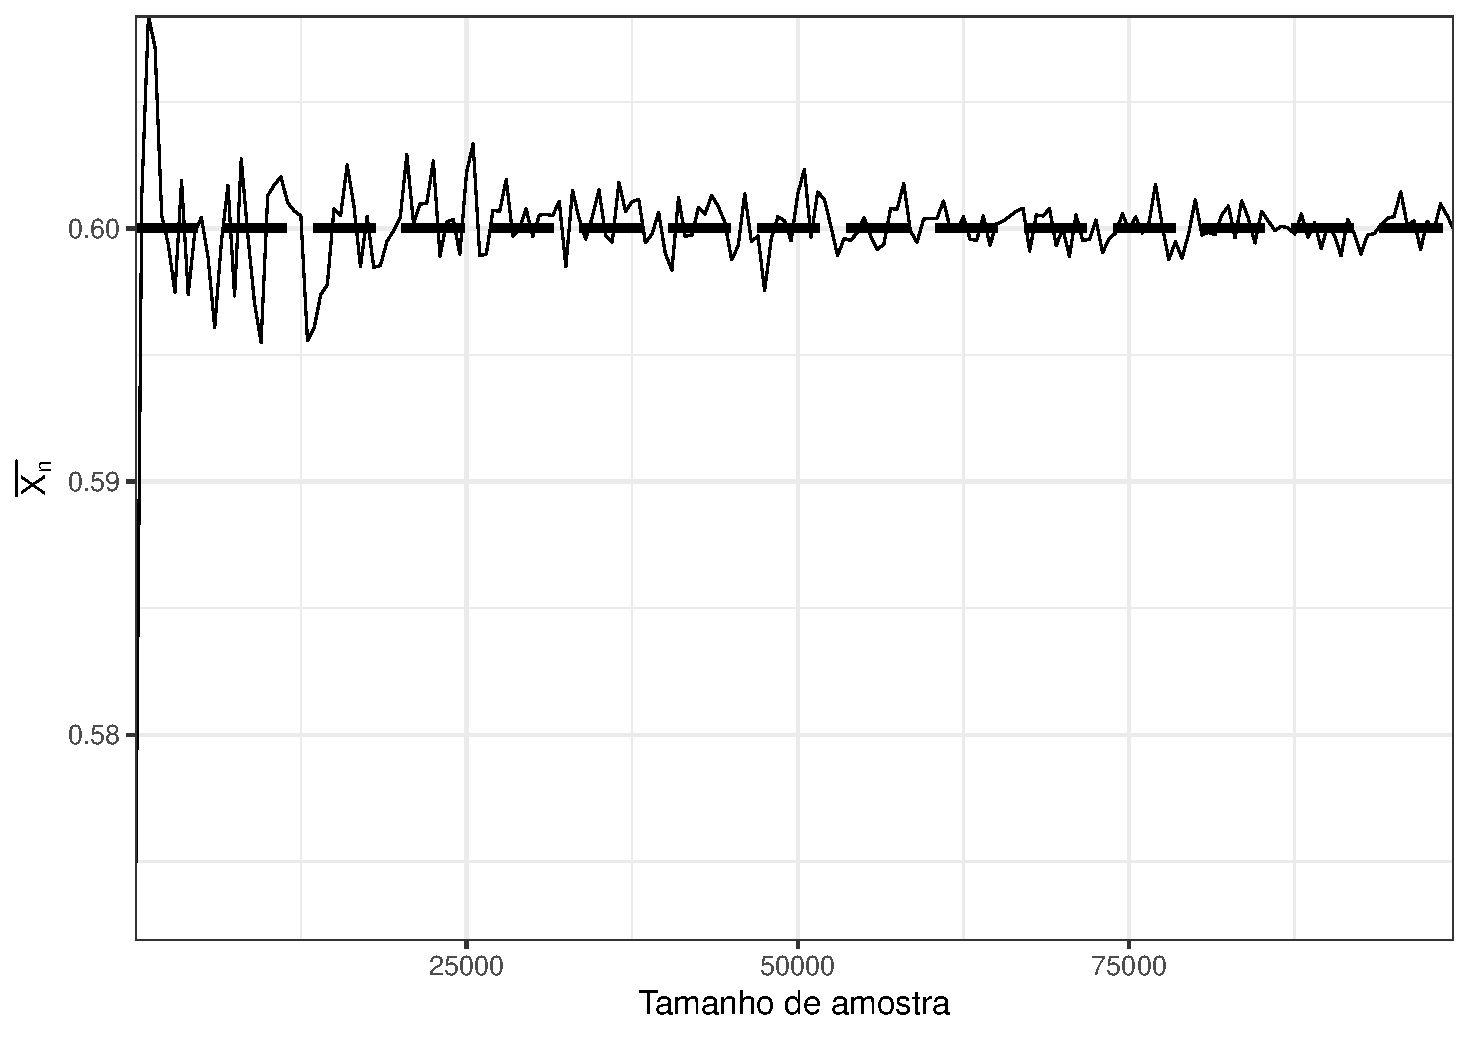
\includegraphics[scale=0.35]{figures/beta_3_2_LGN.pdf} 
\end{center} 
\end{figure} 
\end{frame}
%%%%%%%%%%%%%%%%%%%%%%%%%%%%%%%%%%%
\begin{frame}{Comentário: Lei Forte dos Grandes Números}
\begin{defn}
 \label{dfn:as_convergence}
 \textbf{Convergência quase certa}.
Dizemos que uma sequência de variáveis aleatórias $\left(Z_n\right)_{n\geq 1}$~\textit{converge quase certamente} para $b$ se
$$\pr\left(\lim_{n\to \infty} Z_n = b\right) = 1.$$
\end{defn}
Esse modo de convergência é por vezes chamado de convergência forte.
\textbf{Observação}: convergência quase certa implica convergência em probabilidade.
 \begin{theo}
  \label{thm:SLLN}
  \textbf{Lei forte dos grandes números}
 Sejam  $X_1, X_2, \ldots$ variáveis aleatórias independentes e identicamente distribuídas, com média $\mu$.
 Então
 $$\pr\left(\lim_{n\to \infty} \bar{X}_n = \mu \right) = 1.$$
 \end{theo}
\end{frame}
%%%%%%%%%%%%%%%%%%%%%%%%%%%%%%%%%%%
\begin{frame}[fragile]{Teorema(s) Central(is) do Limite}
O Teorema Central do Limite um dos resultados mais importantes da Estatística.
\begin{theo}
 \label{thm:CLT_LindebergLevy}
\textbf{Teorema Central do Limite} (Lindeberg e Lévy)\footnote{Jarl Waldemar Lindeberg (1876--1932) e Paul Pierre Lévy (1886--1971).}.
Sejam  $X_1, X_2, \ldots, X_n$ variáveis aleatórias independentes e identicamente distribuídas, com média $\mu$ e variância $\sigma^2$.
Então, para cada $x$, temos
$$ \lim_{n\to\infty} \pr\left( \frac{\bar{X}_n - \mu}{\sigma/\sqrt{n}} \leq x \right) = \Phi(x), $$
onde 
$$\Phi(x) := \frac{1}{\sqrt{2\pi}}\int_0^x \exp\left(-\frac{t^2}{2}\right)dt,$$
é a função de distribuição (cumulativa) normal padrão.
\end{theo}
\textbf{Prova}: Ver Casella \& Berger (2002), página 237, teorema 5.5.14.
% Assuma que a função geradora de momentos, $M_X(t)$, existe na vizinhança de zero -- i.e. para $|t| < h, h > 0$.
% 
\end{frame}
%%%%%%%%%%%%%%%%%%%%%%%%%%%%%%%%%%%
\begin{frame}{Teorema Central do Limite: interpretação}
\begin{itemize}
 \item Sabemos que a variável aleatória padronizada $Y_n := \left(\bar{X}_n - \mu\right)/\sigma$ tem média 0 e variância 1, por construção;
 \item O teorema~\ref{thm:CLT_LindebergLevy} nos diz que se tomamos uma amostra grande de uma distribuição com média $\mu$ e variância $\sigma^2$, a variável aleatória $\sqrt{n}Y_n$ terá, aproximadamente, distribuição~\textbf{normal} com média 0 e desvio padrão $1$, chamada~\textit{distribuição normal padrão};
 \item Isto equivale a dizer que $\bar{X}_n \sim \operatorname{normal}(\mu, \sigma^2/n)$;
 \item Note que o teorema vale para~\underline{qualquer} variável aleatória cujos dois primeiros momentos existam, seja ela discreta ou contínua!
\end{itemize}
\end{frame}
%%%%%%%%%%%%%%%%%%%%%%%%%%%%%%%%%%%
\begin{frame}{Teorema Central do Limite: aplicação}
\begin{pergunta}
Suponha que $X_1, \ldots, X_{12}$ são variáveis aleatórias independentes com distribuição uniforme entre 0 e 1.
Defina
$$  p:=  \pr\left(\left| \bar{X}_n - \frac{1}{2}\right| \leq 0.1\right).$$
Quanto vale $p$?
\end{pergunta}
\textbf{Resolução}: 
Lembremos que a variável padronizada $Z = \sqrt{n}(\bar{X}_n-E[X])/\sqrt{\vr(X)}$ terá distribuição aproximadamente normal padrão.
Se $X\sim \operatorname{uniforme}(0, 1)$, sabemos que $E[X] = 1/2$ e $\vr(X) = 1/12$.
Nos aproveitando do fato de que $\sqrt{n}$ e $\sigma$ coincidem nesse exemplo, escrevemos
$$\pr\left(\left| \bar{X}_n - \frac{1}{2}\right| \leq 0.1\right) =  \pr\left(12\left| \bar{X}_n - \frac{1}{2}\right| \leq 0.1\times 12\right) = \pr(|Z| < 1.2),$$
de modo que $p \approx \Phi(1.2)-\Phi(-1.2) = 0.7698607$.
O valor exato, que não discutiremos como obter, é $p = 0.7667213$.
% \footnote{Chebychev diz que $p \geq 1 - 1/(144 \times 0.1^2) \approx 0.31$, o que está longe do valor exato.}
\end{frame}
%%%%%%%%%%%%%%%%%%%%%%%%%%%%%%%%%%%
\begin{frame}{O que aprendemos?}
\begin{itemize}
\item[\faLightbulbO] Desigualdades de Markov e Chebychev: extremamente gerais (mas não muito precisas!);
\item[\faLightbulbO] Convergência fraca (convergência em probabilidade ou medida), $Z \xrightarrow{\text{p}} b$;
\item[\faLightbulbO] Lei (fraca) dos grandes números: a média amostral converge para a média populacional à medida que a amostra aumenta, $\bar{X}_n \xrightarrow{\text{p}} \mu$;
\item[\faLightbulbO] Teorema Central do Limite: para amostras grandes o suficiente, 
$$\bar{X}_n \sim \operatorname{normal}(\mu, \sigma^2/n).$$
\end{itemize} 
\end{frame}
%%%%%%%%%%%%%%%%%%%%%%%%%%%%%%%%%%%
\begin{frame}{Leitura recomendada}
\begin{itemize}
 \item[\faBook] De Groot seções 6.2 e 6.3;
 \item[\faBook] $^\ast$ Casella \& Berger, seções 5.2 e 5.5;
 \item[‡\faGithub] $^\ast$ Nosso repositório (\url{https://github.com/maxbiostat/Statistical_Inference_BSc}).
\end{itemize} 
\end{frame}
